\documentclass[a4paper,oneside,11pt]{article}
\usepackage[T1]{fontenc}     \usepackage[spanish]{babel}
\usepackage[dvips]{graphicx} \usepackage{color}          
\usepackage{amsmath,amscd,amsfonts,amssymb, epsfig,fancyhdr, theorem, fancyhdr}

\pagestyle{fancy}
 \lhead[]{Examen, 17-VI-2008. An�lisis de Estructuras I\\
          E.T.S. Ingenieros de Caminos, Canales y Puertos de Granada}
 \chead[]{} \rhead[\leftmark]{} \cfoot[]{} \lfoot[]{} \rfoot[]{}

\textheight245mm \textwidth170mm \topmargin-15.4mm \oddsidemargin=-5.4mm \headsep10mm

\newcommand{\nombre}{
\noindent\framebox{\parbox{\textwidth}{
\begin{tabular}{ll}
\bf APELLIDOS:\hspace{70mm} & \bf NOMBRE\\*[3mm]
\bf DNI:    & \bf FIRMA:
\end{tabular}}}\bigskip\bigskip}

\newcommand{\problema}[3]{\noindent\textbf{\large\uppercase {#1}}\hfill \large
Tiempo: $#2^{\rm h}\ #3^{\rm
m}$.\bigskip\bigskip}

\newcommand{\f}[2]    {\displaystyle \frac{#1}{#2}}
\newcommand{\al}[0]   {\alpha}

\begin{document}

\nombre

\problema{C�lculo matricial: problema}{2}{00}

\begin{enumerate}
	\item Dada la subestructura compuesta por cinco barras de la figura siguiente, obtener la matriz de rigidez condensado los desplamientos de los nodos 3 y 4, teniendo en cuenta que en dichos nudos no habr� cargas (4 puntos).

		\begin{figure}[hct] \begin{center} 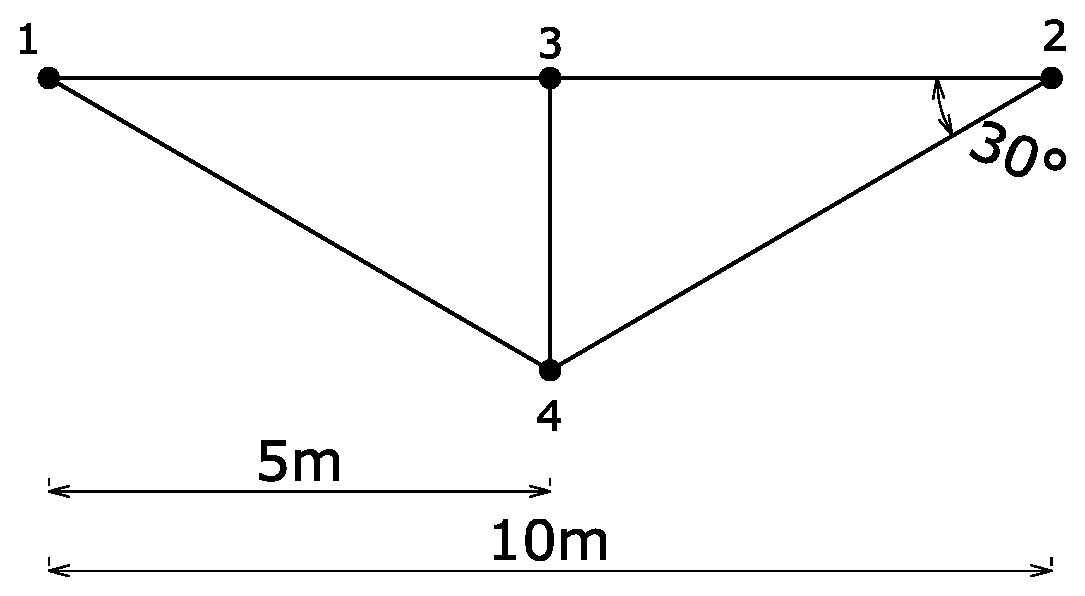
\includegraphics[width=8cm]{../prob_30-06-2008_fig01.eps}\end{center} \end{figure}

	\item Emplear la matriz de rigidez anteriormente obtenida para calcular los desplazamientos en el nodo B de la estructura definida en la figura siguiente considerando las cargas aplicadas (6 puntos).

		\begin{figure}[hct] \begin{center} 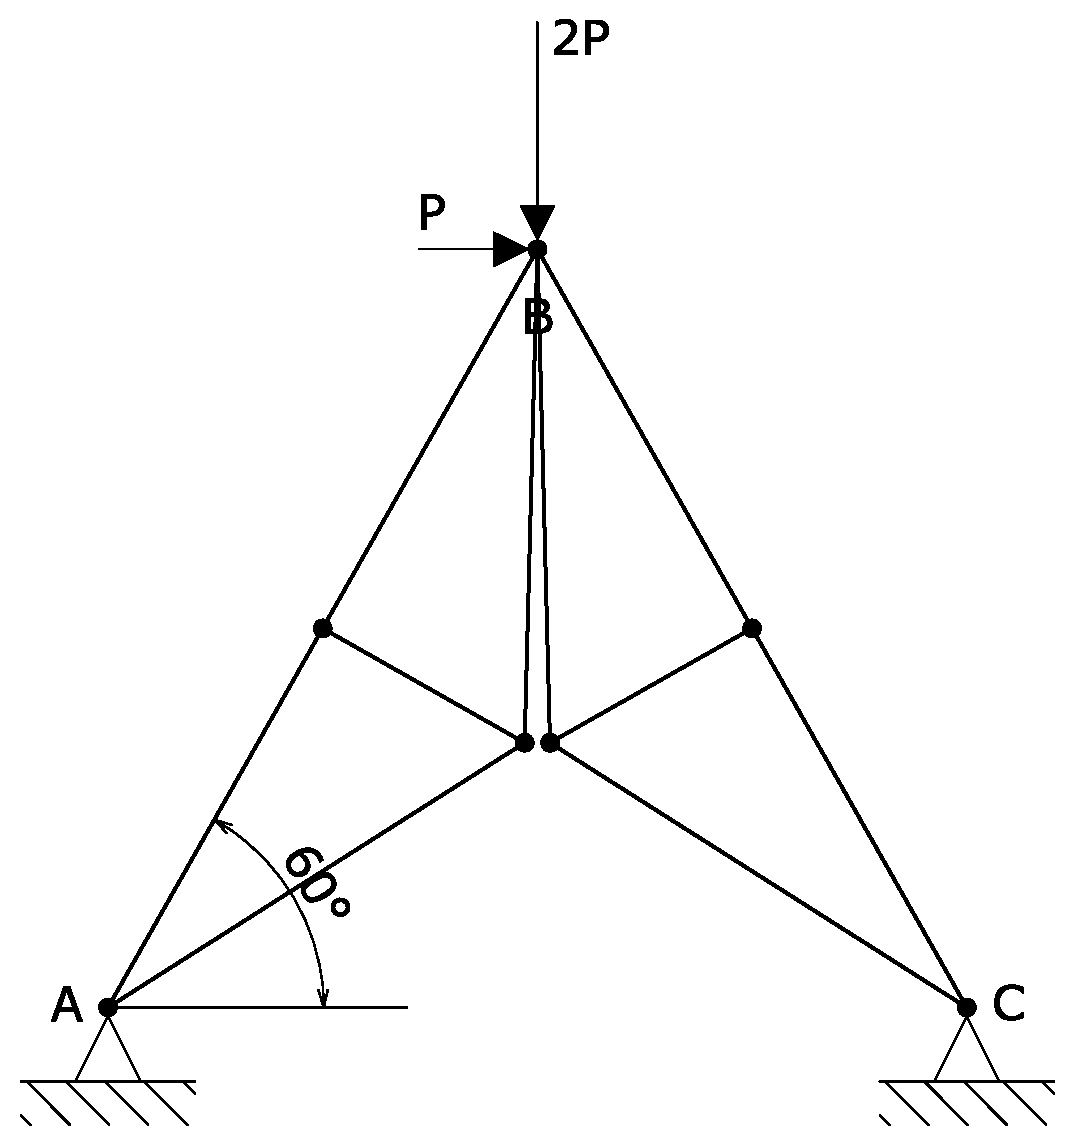
\includegraphics[width=8cm]{../prob_30-06-2008_fig02.eps}\end{center} \end{figure}

\end{enumerate}

(Contin�a)

\newpage

Para el ejercicio 1 siga los pasos siguientes:
\begin{enumerate}
	\item Montaje de la matriz de rigidez completa de la subestructura (8 gdl).
	\item Condensaci�n de los 4 gdl de los nudos 3 y 4 para obtener la matriz solicitada. Para el proceso de condensaci�n se recuerda:
	$\bar{K}_{aa}=K_{aa}-K_{ab} \, K^{-1}_{bb} \, K_{ba}$
\end {enumerate}

Para el ejercicio 2, haga lo siguiente:
\begin{enumerate}
	\item Obtenga la matriz de giro de la subestructura anterior.
	\item Calcule las matrices de rigidez elementales en globales y proceda como en los casos habituales.
\end {enumerate}

Datos: $E=200\,10^{9} {\rm\ N/m^2}$, $I=4.25\,10^{-5} {\rm\ m^4}$, $A=4.25\,10^{-3} {\rm\ m^2}$, $P=10 {\rm\ kN}$.

Nota: No aplique simetr�a en ning�n caso.

Datos para la resoluci�n del problema: D1 = 3, D2 = 0.79, D3 = 0.835

%\nombre

%\problema{C�lculo pl�stico: problema}{0}{45}

%La estructura de nudos r�gidos de la figura se comporta seg�n el modelo r�gido-pl�stico. Calc�lese:
%\begin{itemize}
%\item Factor de carga de colapso.
%\item Distribuci�n de esfuerzos en el momento de colapso.
%\end{itemize}
%Datos: $M_p=30 {\rm\ kNm}$.

%\begin{figure}[hct] \begin{center} \includegraphics[width=10cm]{eps/p060919aei_p}\end{center} \end{figure}

%\problema{C�lculo pl�stico: teor�a}{0}{15}

%Responda sint�tica y brevemente a las siguientes cuestiones:
%\begin{enumerate}
%\item ?`De qu� depende que la zona plastificada tenga forma parab�lica o triangular?
%\item En la formulaci�n general de problemas de optimizaci�n, ?`Porqu� las restricciones adoptan la forma de desigualdades?
%\end{enumerate}

\end{document}

